\documentclass[letterpaper,10pt]{amsart}

\usepackage[pdftex]{graphicx}
\usepackage{moreverb}
\usepackage{amsmath}
\usepackage{amsthm}
\usepackage{fullpage}
\usepackage{amssymb}
\usepackage{tikz}
\usepackage{dsfont}
\usepackage{hyperref}
\usepackage[all]{xy}
\usepackage{bbm}
\usepackage{mathtools}
\usepackage[margin=0.5in]{geometry}
\usepackage{enumerate}
\usepackage{multirow}
\usepackage{cancel}


\newcommand{\sumin}{\sum_{i=1}^n}
\newcommand{\sumjn}{\sum_{j=1}^n}
\newcommand{\sumiN}{\sum_{i=1}^N}
\newcommand{\sumjN}{\sum_{j=1}^N}
\newcommand{\sumim}{\sum_{i=1}^m}
\newcommand{\sumjm}{\sum_{j=1}^m}
\newcommand{\prodin}{\prod_{i=1}^n}
\newcommand{\rmd}{\mathrm{d}}
\newcommand{\dx}{\,\mathrm{d}x}
\newcommand{\dy}{\,\mathrm{d}y}
\newcommand{\dt}{\,\mathrm{d}t}
\newcommand{\dz}{\,\mathrm{d}z}
\newcommand{\dmu}{\,\mathrm{d}\mu}
\newcommand{\dnu}{\,\mathrm{d}\nu}
\newcommand{\dP}{\,\mathrm{d}\mathbb{P}}
\newcommand{\fa}{\; \forall \;}


%distributions and functions
\newcommand{\E}[1]{\mathbb{E}\!\left[#1\right]}
\newcommand{\Esub}[2]{\mathbb{E}_{#1}\left[#2\right]}
\newcommand{\p}[1]{\mathbb{P}\!\left(#1\right)}
\newcommand{\psub}[2]{\mathbb{P}_{#1}\left(#2\right)}
\newcommand{\tr}{\operatorname{tr}}
\newcommand{\Var}{\operatorname{Var}}
\newcommand{\Cov}{\operatorname{Cov}}
\newcommand{\Corr}{\operatorname{Corr}}
\newcommand{\argmax}{\operatorname*{arg \, max}}
\newcommand{\argmin}{\operatorname*{arg \, min}}
\newcommand{\Beta}{\textnormal{Beta}}
\newcommand{\Bin}{\textnormal{Bin}}
\newcommand{\logit}{\operatorname{logit}}
\newcommand{\Gammadist}{\textnormal{Gamma}}
\newcommand{\Geom}{\textnormal{Geom}}
\newcommand{\Expo}{\textnormal{Expo}}
\newcommand{\Pois}{\textnormal{Pois}}
\newcommand{\Unif}{\textnormal{Uniform}}
\newcommand{\Bern}{\textnormal{Bern}}
\newcommand{\sgn}{\operatorname{sgn}}
\newcommand{\Mult}{\textnormal{Mult}}
\newcommand{\MVN}{\textnormal{MVN}}


%special letters
\newcommand{\sA}{\mathcal{A}}
\newcommand{\sB}{\mathfrak{B}}
\newcommand{\sC}{\mathcal{C}}
\newcommand{\sD}{\mathcal{D}}
\newcommand{\sF}{\mathcal{F}}
\newcommand{\sG}{\mathcal{G}}
\newcommand{\sH}{\mathcal{H}}
\newcommand{\sI}{\mathcal{I}}
\newcommand{\sL}{\mathcal{L}}
\newcommand{\sP}{\mathcal{P}}
\newcommand{\sQ}{\mathbb{Q}}
\newcommand{\sR}{\mathbb{R}}
\newcommand{\sS}{\mathcal{S}}
\newcommand{\sT}{\mathcal{T}}
\newcommand{\sX}{\mathcal{X}}
\newcommand{\indep}{\perp\!\!\!\perp}
\newcommand{\io}{\text{ i.o.}}

\newtheorem*{prop}{Prop}
\newtheorem{theorem}{Theorem}
\newtheorem*{claim}{Claim}
\newtheorem*{corollary}{Corollary}
\newtheorem{defn}{Definition}
\newtheorem{ex}{Example}
\newtheorem*{lemma}{Lemma}
\newtheorem*{exercise}{Exercise}

\newenvironment{verbatimcode}{\bigskip \scriptsize \verbatim}{\endverbatim \normalsize \bigskip}
\allowdisplaybreaks

\begin{document}

\title{STAT 221 - Assignment 3}
\author{Greg Tam, Student ID: 70908239}
\date{}
\maketitle


\begin{enumerate}[1.]
\item
\begin{enumerate}[(a)]
\item
By Adam's law, we have that
\begin{align*}
\E{y_n | \boldsymbol x_n} &= \E{\E{y_n | \lambda_n} | \boldsymbol x_n}\\
&= \E{h(\lambda_n) | \boldsymbol x_n}\\
&= \E{h(\boldsymbol x_n' \boldsymbol \theta^*) | \boldsymbol x_n}\\
&= h(\boldsymbol x_n' \boldsymbol \theta^*)
\end{align*}
Now consider
\[f(y_n | \lambda_n) = \exp\left\{\frac{\lambda_n y_n - b(\lambda_n)}{\phi}\right\} \cdot c(y_n, \phi)\]
Taking logs, we get
\[\ell(\lambda_n) = \log f(y_n | \lambda_n) = \frac{\lambda_n y_n - b(\lambda_n)}{\phi} + \log c(y_n, \phi)\]
Then differentiating, we get
\[\ell'(\lambda_n) = \frac{y_n - b'(\lambda_n)}{\phi}\]
Taking expectations on both sides and using the fact that $\E{\ell'(\lambda_n)}=0$, we have
\[\E{\frac{y_n - b'(\lambda_n)}{\phi}}=0\]
which implies
\[\E{y_n | \lambda_n} = b'(\lambda_n)\]
Using the same logic as above, we have
\begin{align*}
\E{y_n | \boldsymbol x_n} &= \E{\E{y_n | \lambda_n} | \boldsymbol x_n}\\
&= \E{b'(\lambda_n) | \boldsymbol x_n}\\
&= \E{b'(\boldsymbol x' \boldsymbol \theta^*) | x_n}\\
&= b'(\boldsymbol x' \boldsymbol \theta^*)\\
&= b'(\lambda_n)
\end{align*}


\item For this part, we will use the the fact that under regularity conditions, we have
\[\E{-\ell''(\lambda_n)} = \E{\{\ell'(\lambda_n)\}^2}\]
Recall that
\[\ell'(\lambda_n) = \frac{y_n - b'(\lambda_n)}{\phi}\]
Differentiating once more, we get
\[\ell''(\lambda_n) = -\frac{b''(\lambda_n)}{\phi}\]
So this gives us
\begin{align*}
\E{\frac{b''(\lambda_n)}{\phi}} &= \E{\left(\frac{y_n - b'(\lambda_n)}{\phi}\right)^2}\\
&= \E{\frac{y_n^2 - 2 y_n b'(\lambda_n) + \{b'(\lambda_n)\}^2}{\phi^2}}
\end{align*}
By linearity of expectation, we have
\[\frac{b''(\lambda_n)}{\phi} = \frac{\E{y_n^2 | \lambda_n} - 2\E{y_n | \lambda_n} b'(\lambda_n) + \{b'(\lambda_n)\}^2}{\phi^2}\]
Now, using the fact that $\E{y_n | \lambda_n} = b'(\lambda_n)$, we get the middle term
\[2\E{y_n | \lambda_n}b'(\lambda_n) = \E{y_n | \lambda_n}^2 + \{b'(\lambda_n)\}^2\]
Substituting this in, we get
\begin{align*}
\frac{b''(\lambda_n)}{\phi} &= \frac{\E{y_n^2 | \lambda_n} - \{\E{y_n | \lambda_n}\}^2 - \{b'(\lambda_n)^2\} + \{b'(\lambda_n)\}^2}{\phi^2}\\
&= \frac{\E{y_n^2 | \lambda_n} - \{\E{y_n | \lambda_n}\}^2}{\phi^2}\\
&= \frac{\Var(y_n | \lambda_n)}{\phi^2}
\end{align*}
and so
\[\Var(y_n | \lambda_n) = \phi \cdot b''(\lambda_n) = \phi \cdot h'(\lambda_n)\]

\item
We have that 
\begin{align*}
f(y_n | \lambda_n) &= \exp\left\{\frac{\lambda_n y_n - b(\lambda_n)}{\phi}\right\} \cdot c(y_n, \phi)\\
&= \exp\left\{\frac{\boldsymbol x_n' \boldsymbol \theta^* y_n - b(\boldsymbol x_n' \boldsymbol \theta^*)}{\phi}\right\} \cdot c(y_n, \phi)
\end{align*}
Taking logs, we get
\[\ell(\theta; y_n, \boldsymbol x_n) = \frac{\boldsymbol x_n' \boldsymbol \theta^* y_n - b(\boldsymbol x_n' \boldsymbol \theta^*)}{\phi}  + \log c(y_n, \phi)\]
This gives
\begin{align*}
\nabla \ell(\theta; y_n, \boldsymbol x_n) &= \frac{y_n \boldsymbol x_n - b'(\boldsymbol x_n' \boldsymbol \theta^*) \boldsymbol x_n}{\phi}\\
&= \frac{1}{\phi}\left\{y_n - h(\boldsymbol x_n' \boldsymbol \theta^*)\right\} \boldsymbol x_n
\end{align*}

\item
By definition, we have
\[\left(\sI(\boldsymbol \theta)\right)_{i,j} = -\E{\frac{\partial^2}{\partial \boldsymbol \theta_i \partial \boldsymbol \theta_j} \ell(\boldsymbol \theta; y_n, \boldsymbol x_n)}\]
for each index $i,j$. It follows trivially that
\[\sI(\boldsymbol \theta) = -\E{\nabla \nabla \ell(\boldsymbol \theta; y_n, \boldsymbol x_n)}\]
Next, we have
\begin{align*}
\nabla \nabla \ell(\boldsymbol \theta; y_n, \boldsymbol x_n) &= \nabla \left\{\frac{1}{\phi}(y_n - h(\boldsymbol x_n' \boldsymbol \theta^*) \boldsymbol x_n\right\}\\
&= -\frac{\left\{0+h'(\boldsymbol x_n' \boldsymbol \theta^*)\right\} \boldsymbol x_n \boldsymbol x_n'}{\phi}\\
&= - \frac{h'(\boldsymbol x_n' \boldsymbol \theta^*) \boldsymbol x_n \boldsymbol x_n'}{\phi}
\end{align*}
Multiplying by $-1$ and taking expectations yields our result: 
\[\sI(\boldsymbol \theta) = -\E{\nabla \nabla \ell(\boldsymbol \theta; y_n, \boldsymbol x_n)} = \frac{1}{\phi}\E{h'(\boldsymbol x_n' \boldsymbol \theta^*) \boldsymbol x_n \boldsymbol x_n'} \]



\item
We can show that $h(\cdot )$ is non-decreasing by looking at $\Var(y_n | \lambda_n)$. Recall that $\Var(y_n | \lambda_n) = \phi \cdot h'(\lambda_n)$. We are given that $\phi > 0$ and we know
\[\Var(y_n | \lambda_n = \phi \cdot h'(\lambda_n) \geq 0\]
since it is a variance. hence, we have $h'(\lambda_n) \geq 0$, which implies that $h(\cdot)$ is non-decreasing.
\end{enumerate}


\item
\begin{enumerate}[(a)]
\item

The function we wish to minimize is $\Esub{x}{(\theta - x)' A(\theta - x)}$. 
\begin{itemize}
\item 
To do this for SGD, we can take iterates
\begin{align*}
\boldsymbol \theta_{t+1} &= \boldsymbol \theta_t - \gamma_t \nabla (\boldsymbol \theta_t - \boldsymbol x_t)' A (\boldsymbol \theta_t - \boldsymbol x_t)\\
&= \boldsymbol \theta_t - \gamma_t 2A(\boldsymbol \theta_t - \boldsymbol x_t)
\end{align*}
\item 
In the case of ASGD, do the same iteration, but instead of taking $\boldsymbol \theta_{t+1}$, we take $\bar{\boldsymbol \theta}_{t+1} = \frac{1}{t+1} \sum_{j=1}^{t+1} \boldsymbol \theta_j$, as our result. 
\item
For the implicit case, we need to solve $\boldsymbol \theta_{t+1} = \boldsymbol \theta_t - \gamma_t 2A(\boldsymbol \theta_{t+1} - \boldsymbol x_t)$. Moving the last term on the right to the left hand side, we get
\[\boldsymbol \theta_{t+1} + \gamma_t 2A(\boldsymbol \theta_{t+1} - x_t) = \boldsymbol \theta_t\]
Then we can factor the $\boldsymbol \theta_{t+1}$ vector out.
\[(I + \gamma_t 2A)\boldsymbol \theta_{t+1} = \boldsymbol \theta_t + \gamma_t 2A \boldsymbol x_t\]
Finally, we multiply both sides by $(I + \gamma_t 2 A)^{-1}$.
\[\boldsymbol \theta_{t+1} = (I + \gamma_t 2A)^{-1}(\boldsymbol \theta_t + \gamma_t 2 A \boldsymbol x_t)\]
\end{itemize}

When we run our code, we get the follow plot
\begin{center}
\includegraphics[scale=0.8]{221Ass3-Q2-a.png}
\end{center}


\item
We have that $y_n | \lambda_n \sim \mathcal{N}(\lambda_n, \sigma^2)$, $\lambda_n = \boldsymbol x_n' \boldsymbol \theta^*$ and $\boldsymbol \theta^* \in \sR^p$.
For this part, we are required to find $\min_{\boldsymbol \theta} (y - \boldsymbol x_n' \boldsymbol \theta)^2$ as this determines the best $\boldsymbol \theta$ parameter because this is a linear regression. We have that $\ell(\boldsymbol \theta;y_t, \boldsymbol x_t) = (y_t  - \boldsymbol x_t' \boldsymbol \theta)^2$. 


\begin{itemize}
\item
Our SGD is defined by
\begin{align*}
\boldsymbol \theta_{t+1} &= \boldsymbol \theta_t - \gamma_t \nabla (y_t - \boldsymbol x_t'\boldsymbol \theta_t)^2\\
&= \boldsymbol \theta_t - \gamma_t 2(y_t - \boldsymbol  x_t' \boldsymbol \theta_t) \boldsymbol x_t\\
&= \boldsymbol \theta_t + \alpha_t (y_t - \boldsymbol x_t' \boldsymbol \theta_t)\boldsymbol x_t
\end{align*}
where $\alpha_t = -2\gamma_t$.


\item

As before, we can get the ASGD by doing a simple modification to this by simply take $\bar{\boldsymbol \theta}_{t+1}$ instead of $\boldsymbol \theta_{t+1}$,

\item
For the implicit case, we need to solve
\[\boldsymbol \theta_{t+1} = \boldsymbol \theta_t + \alpha _t y_t \boldsymbol x_t - \alpha_t \boldsymbol x_t' \boldsymbol \theta_{t+1} \boldsymbol x_t\]
We move the $\alpha_t \boldsymbol x_t' \boldsymbol \theta_{t+1} \boldsymbol x_t$ term to the left hand side, which gives us
\[\boldsymbol \theta_{t+1} + \alpha_t \boldsymbol x_t' \boldsymbol \theta_{t+1} \boldsymbol x_t = \boldsymbol \theta_t + \alpha_t y_t \boldsymbol x_t\]
Since $\boldsymbol x_t' \boldsymbol \theta_{t+1}$ is simply a scalar quantity, we can move it to give
\[\boldsymbol \theta_{t+1} + \alpha_t  \boldsymbol x_t \boldsymbol x_t' \boldsymbol \theta_{t+1}= \boldsymbol \theta_t + \alpha_t y_t \boldsymbol x_t\]
Factoring out the $\boldsymbol \theta_{t+1}$ vector gives
\[(I + \alpha_t \boldsymbol x_t \boldsymbol x_t') \boldsymbol \theta_{t+1} = \boldsymbol \theta_t + \alpha_t y_t \boldsymbol x_t\]
Then multiplying both sides by $(I + \alpha_t \boldsymbol x_t \boldsymbol x_t')^{-1}$ gives
\[\boldsymbol \theta_{t+1} = (I + \alpha_t \boldsymbol x_t \boldsymbol x_t')^{-1} (\boldsymbol \theta_t + \alpha_t y_t \boldsymbol x_t)\]
To get this inverse, we apply the Sherman-Morrison formula which states that
\[(A + uv')^{-1} = A^{-1} - \frac{A^{-1} uv' A^{-1}}{1 + v'A^{-1} u}\]
Now, we have 
\begin{align*}
(I + \alpha_t \boldsymbol x_t \boldsymbol x_t')^{-1} &= \frac{1}{\alpha_t}\left(\frac{1}{\alpha_t}I + \boldsymbol x_t \boldsymbol x_t' \right)^{-1}\\
&= \frac{1}{\alpha_t}\left(\alpha_t I - \frac{\alpha_t I \boldsymbol x_t \boldsymbol x_t' \alpha_t I}{1 + \boldsymbol x_t' \alpha_t I \boldsymbol x_t}\right) \qquad \text{by Sherman-Morrison}\\
&= \frac{1}{\alpha_t} \left(\alpha_t I - \frac{\alpha_t^2 \boldsymbol x_t \boldsymbol x_t'}{1 + \alpha_t \boldsymbol x_t' \boldsymbol x_t}\right)\\
&= I - \frac{\alpha_t \boldsymbol x_t \boldsymbol x_t'}{1 + \alpha_t \|\boldsymbol x_t\|^2}
\end{align*}
Using this, we have
\begin{align*}
\boldsymbol \theta_{t+1} &= \left(I - \frac{\alpha_t \boldsymbol x_t \boldsymbol x_t'}{1 + \alpha_t \|\boldsymbol x_t\|^2}\right) (\boldsymbol \theta_t + \alpha_t y_t \boldsymbol x_t)\\
&= \boldsymbol \theta_t + \alpha_t y_t \boldsymbol x_t - \frac{\alpha_t (\boldsymbol x_t' \boldsymbol \theta_t) \boldsymbol x_t}{1 + \alpha_t \|\boldsymbol x_t\|^2} - \frac{\alpha_t^2 y_t \|\boldsymbol x_t\|^2 \boldsymbol x_t}{1 + \alpha_t \|\boldsymbol x_t\|^2}
\end{align*}
\end{itemize}
Our plots are shown below: 
\begin{center}
\includegraphics[scale=0.8]{2bold.png}
\end{center}

Note: I had some strange issues with the ASGD, which I couldn't figure out how to fix. The ASGD is a simple modification of the SGD. Once we calculate $\theta_{t+1}$ given $\theta_t$, instead of returning $\theta_{t+1}$, we return the average of $\theta_1,\ldots,\theta_{t+1}$. That is, 
\[\theta_{t+1} = \frac{t\bar{\theta}_t  + \theta_{t+1}}{t+1} \]

\item 
The plots of the bias and the variances for the methods SGD, ASGD, and Implicit are as follows: For the bias term, I used the metric 
\[\|\theta_n - \theta^*\| = \log((\theta_n - \theta^*)'(\theta_n - \theta^*)) \]
where $\theta* = \boldsymbol 1$, that is, it is a vector of ones.
\begin{center}
\includegraphics[scale=0.4]{2cbias1.pdf}
\includegraphics[scale=0.4]{2cbias2.pdf}
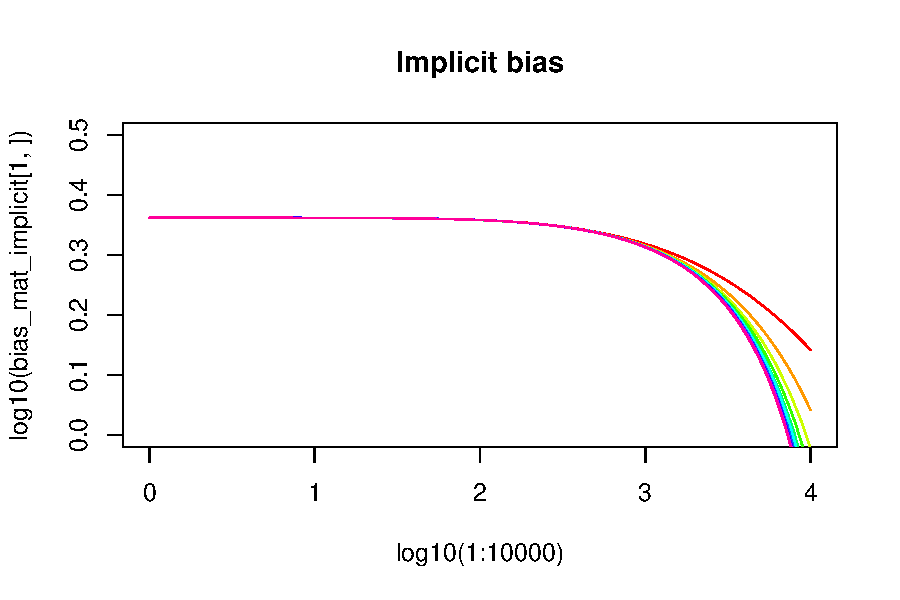
\includegraphics[scale=0.4]{2cbias3.pdf}
\end{center}

Again, I ran into issues with the ASGD. I ran this across $10^4$ iterations locally and it had more risk that the other methods. I then tried to run it anyway for more iterations to see if it would lower in the long term, but for some reason something bizarre happened and it did not perform like it should.



\item
Our variance plots are as follows. In order to plot this, a one dimensional summary of each variance-covariance matrix was used. In this case, we used $\tr(\Var(\theta_n))$.
\begin{center}
\includegraphics[scale=0.4]{2cvar1.pdf}
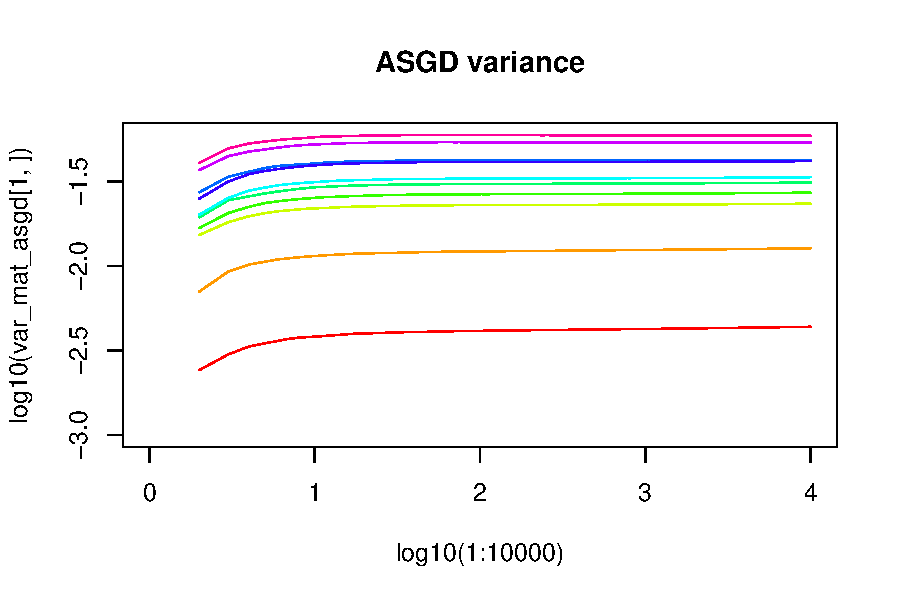
\includegraphics[scale=0.4]{2cvar2.pdf}
\includegraphics[scale=0.4]{2cvar3.pdf}
\end{center}
Again, we have the same caveat that something went wrong in the ASGD.

\item
We have that 
\[y_n | x_n, \theta^* \sim \mathcal{N}(x_n' \theta^*, \sigma^2)\]
This has density
\[f_{Y_n}(y_n) = \frac{1}{\sqrt{2 \pi \sigma^2}}e^{}-\frac{(y_N - x_n'\theta^*)^2}{2\sigma^2}\]
Taking logs, we get
\[\log f_{Y_n}(y_n) = \log\left(\frac{1}{\sqrt{2 \pi \sigma^2}}\right) - \frac{(y_n - x_n' \theta^*)^2}{2\sigma^2}  \]
Taking the partial derivative with respect to $\theta$, we get
\begin{align*}
\frac{\partial}{\partial \theta} \log f_{Y_n}(y_n) &= \frac{2(y_n - x_n' \theta^*)x_n}{2 \sigma^2}\\
&= \frac{(y_n - x_n' \theta^*) x_n}{\sigma^2}
\end{align*}
and so the Fisher Information matrix is
\begin{align*}
\sI(\theta^*) &= \E{\left(\frac{\partial}{\partial \theta} \log f_{Y_n}(y_n)\right)\left(\frac{\partial}{\partial \theta} \log f_{Y_n}(y_n)\right)'}\\
&= \E{\frac{(y_n - x_n' \theta)^2}{\sigma^4} x_n x_n'}\\
&= \frac{x_n x_n' }{\sigma^4} \E{(y_n - x_n' \theta)^2}\\
&= \frac{x_n x_n' }{\sigma^4} \sigma^2\\
&= \frac{x_n x_n'}{\sigma^2}
\end{align*}
\end{enumerate}


\item
\begin{enumerate}[(a)]
\item
The elastic net is an algorithm which encompasses both lasso and ridge regression. It is a more general form which solves the problem 
\[\min_{(\beta_0,\beta) \sin \sR^{p+1}} R_\lambda (\beta_0, \beta) = \min_{(\beta_0, \beta) \in \sR^{p+1}} \left[\frac{1}{2N}\sum_{i=1}^N (y_i - \beta_0 - x_i' \beta)^2 + \lambda P_{\alpha}(\beta)\right]\] 
where
\begin{align*}
P_{\alpha}(\beta) &= (1-\alpha)\frac{1}{2}\|\beta\|_{\ell_2}^2 + \alpha \|\beta\|_{\ell_1}\\
&= \sum_{j=1}^p \left[\frac{1}{2}(1-\alpha)\beta_j^2 + \alpha | \beta_j|\right]
\end{align*}
The algorithm \texttt{glmnet} exploits sparcity through the use of $P_\alpha$. This penalty term is a compromise between the ridge-regression penalty, when $\alpha=0$, and the lasso penalty, when $\alpha=1$. Increasing $\alpha$ increases the number of coefficients equal to zero, and hence the sparcity increases, making calculations run faster.

\item
Using Panos' \texttt{glmnet.R} code and then running
\begin{verbatimcode}
times = matrix(,nrow=0,ncol=6)
params = cbind(N=c(1000,5000,100,100,100,100), p=c(100,100,1000,5000,20000,50000))
for(i in 1:6)
{
  N = params[i,"N"]
  p = params[i,"p"]
  ans = run.glmnet(N, p,type="naive")
  ans2 = run.glmnet(N, p,type="covariance")
  times = rbind(times,tapply(ans[,"time"],c(rep(1,6),rep(2,6),rep(3,6)), mean))
  times = rbind(times,tapply(ans2[,"time"],c(rep(1,6),rep(2,6),rep(3,6)), mean))
}
times
\end{verbatimcode}
we get the table:
\begin{center}
\begin{tabular}{lrrrrrr}
 & \multicolumn{6}{c}{\text{Linear regression - Dense features}} \\ \cline{2-7}
 & & & & & & \\
 & \multicolumn{6}{c}{\text{Correlation}} \\
 & 0 & 0.1 & 0.2 & 0.5 & 0.9 & 0.95  \\ \cline{2-7}
 & & & & & & \\
 & \multicolumn{6}{c}{$N=1000,p=100$}\\ \cline{2-7}
\texttt{glmnet (type="naive")} & 0.09383333 & 0.07866667 & 0.07500000 & 0.09383333 & 0.07866667 & 0.07500000\\
\texttt{glmnet (type="cov")} & 0.01300000 & 0.01433333 & 0.01350000 & 0.01300000 & 0.01433333 & 0.01350000\\ \cline{2-7}
 & & & & & & \\
 & \multicolumn{6}{c}{$N=5000,p=100$}\\ \cline{2-7}
\texttt{glmnet (type="naive")} & 0.28583333 & 0.32300000 & 0.34333333 & 0.28583333 & 0.32300000 & 0.34333333\\
\texttt{glmnet (type="cov")} & 0.03900000 & 0.03833333 & 0.03633333 & 0.03900000 & 0.03833333 & 0.03633333\\ \cline{2-7}
 & & & & & & \\
 & \multicolumn{6}{c}{$N=100,p=1000$}\\ \cline{2-7}
\texttt{glmnet (type="naive")} & 0.03366667 & 0.03633333 & 0.03300000 & 0.03366667 & 0.03633333 & 0.03300000\\
\texttt{glmnet (type="cov")} & 0.07016667 & 0.07216667 & 0.06050000 & 0.07016667 & 0.07216667 & 0.06050000\\ \cline{2-7}
 & & & & & & \\
 & \multicolumn{6}{c}{$N=100,p=5000$}\\ \cline{2-7}
\texttt{glmnet (type="naive")} & 0.14050000 & 0.09366667 & 0.09700000 & 0.14050000 & 0.09366667 & 0.09700000\\
\texttt{glmnet (type="cov")} & 0.37366667 & 0.32083333 & 0.33233333 & 0.37366667 & 0.32083333 & 0.33233333\\ \cline{2-7}
 & & & & & & \\
 & \multicolumn{6}{c}{$N=100,p=20000$}\\ \cline{2-7}
\texttt{glmnet (type="naive")} & 0.32933333 & 0.34200000 & 0.38166667 & 0.32933333 & 0.34200000 & 0.38166667\\
\texttt{glmnet (type="cov")} & 1.49150000 & 1.43166667 & 1.45516667 & 1.49150000 & 1.43166667 & 1.45516667\\ \cline{2-7}
 & & & & & & \\
 & \multicolumn{6}{c}{$N=100,p=50000$}\\ \cline{2-7}
\texttt{glmnet (type="naive")} & 0.74233333 & 0.76333333 & 0.88183333 & 0.74233333 & 0.76333333 & 0.88183333\\
\texttt{glmnet (type="cov")} & 3.31166667 & 3.83350000 & 4.49833333 & 3.31166667 & 3.83350000 & 4.49833333\\ \cline{2-7}
\end{tabular}
\end{center}
\bigskip


\item 
After running the SGD for each set of $N$ and $p$ values, we get the following results.

\bigskip

\begin{center}
\begin{tabular}{lrrrrrr}
 & \multicolumn{6}{c}{\text{Linear regression - Dense features}} \\ \cline{2-7}
 & & & & & & \\
 & \multicolumn{6}{c}{\text{Correlation}} \\
 & 0 & 0.1 & 0.2 & 0.5 & 0.9 & 0.95  \\ \cline{2-7}
 & & & & & & \\
 & \multicolumn{6}{c}{$N=1000,p=100$}\\ \cline{2-7}
\texttt{SGD} & 0.31100000 & 0.2986667 & 0.30866667 & 0.30900000 & 0.31500000 & 0.33233333\\ \cline{2-7}
 & & & & & & \\
 & \multicolumn{6}{c}{$N=5000,p=100$}\\ \cline{2-7}
\texttt{SGD} & 7.09300000 & 7.2303333 & 7.16200000 & 7.29366667 & 7.32633333 & 7.67033333\\ \cline{2-7}
 & & & & & & \\
 & \multicolumn{6}{c}{$N=100,p=1000$}\\ \cline{2-7}
\texttt{SGD} & 0.03933333 & 0.0370000 & 0.03666667 & 0.03666667 & 0.04033333 & 0.03766667\\ \cline{2-7}
 & & & & & & \\
 & \multicolumn{6}{c}{$N=100,p=5000$}\\ \cline{2-7}
\texttt{SGD} & 0.37600000 & 0.3633333 & 0.39733333 & 0.29366667 & 1.28133333 & 1.38033333\\ \cline{2-7}
 & & & & & & \\
 & \multicolumn{6}{c}{$N=100,p=20000$}\\ \cline{2-7}
\texttt{SGD} & 2.45833333 & 1.8180000 & 1.51933333 & 1.52100000 & 1.56833333 & 1.58300000\\ \cline{2-7}
 & & & & & & \\
 & \multicolumn{6}{c}{$N=100,p=50000$}\\ \cline{2-7}
\texttt{SGD} & 3.48600000 & 3.4553333 & 3.49833333 & 3.55466667 & 3.54500000 & 3.63233333\\ \cline{2-7}
\end{tabular}
\end{center}
\bigskip
We can see that SGD is a lot slower than the naive case of \texttt{glmnet}. When $N=100$, the cov case of \texttt{glmnet} runs quicker, but SGD is a slower when there are more iterations as shown in the $N=1000$ and $N=5000$ cases. 


\item 
When I run this part, I do a very slight modiciation fo part (c). 
\begin{verbatimcode}
times = matrix(,nrow=0,ncol=6)

start_time = Sys.time()
task.id = as.numeric(Sys.getenv("SLURM_ARRAY_TASK_ID"))
job.id = as.numeric(Sys.getenv("SLURM_ARRAY_JOB_ID"))
print(paste("task.id ", task.id,"   ---  job.id  ",job.id))
N = 50000
p = 10e3
ans = run.glmnet(N, p)
times = rbind(times,tapply(ans[,"time"],c(rep(1,3),rep(2,3),rep(3,3),rep(4,3),rep(5,3),rep(6,3)), mean))
end_time = Sys.time()
total_time = as.numeric(end_time-start_time,units="mins")

save(list=c("times","start_time","end_time","total_time"),file=sprintf("odyssey/pset3/3d_job%d_task%d.rda", job.id, task.id))
\end{verbatimcode}
Unfortunately, due to time constraints, my file wasn't able to complete. It had run at $N=50000$ for over 9 hours. Every iteration increases the amount of computational time required exponentially in an SGD. As to expect, the times for each of the SGDs with different correlations are expected to be large. 
\end{enumerate}

\end{enumerate}


\end{document}

